\documentclass[a4paper,10pt]{article}
\topmargin-1cm
\addtolength{\textheight}{2.5cm}
\addtolength{\textwidth}{2cm}
\usepackage{times}

\usepackage{verbatim}
\usepackage[dvips]{graphicx}
\usepackage[german]{babel}
\usepackage[latin1]{inputenc}

\setlength{\parindent}{0cm}

\title{Latex Template}
\author{David Herzig}
\date{WS2013}

\begin{document}

HF-ICT - H"ohere Fachschule f"ur Informations- und Kommunikationstechnologie\\
CH 4132 Muttenz\\
D.Herzig

\vspace{2mm}

\begin{center}
{\Large \bf Vorkurs Informatik}\\
Exercise sheet 9
\end{center}

\vspace{2mm}

\line(1,0){400}

\vspace{5mm}

\section{Galtonsches Brett}
Das Galtonsche Brett ist ein vertikales Brett mit N"ageln, an welchen herunterfallende Kugeln abgelenkt werden. Die N"agel sind in r=5 horizontalen Reihen angeordnet, sodass eine fallende Kugel bei jeder Reihe zuf"allig nach links oder rechts abgelenkt wird, bis sie unten in ein Fach f"allt.

\vspace{5mm}

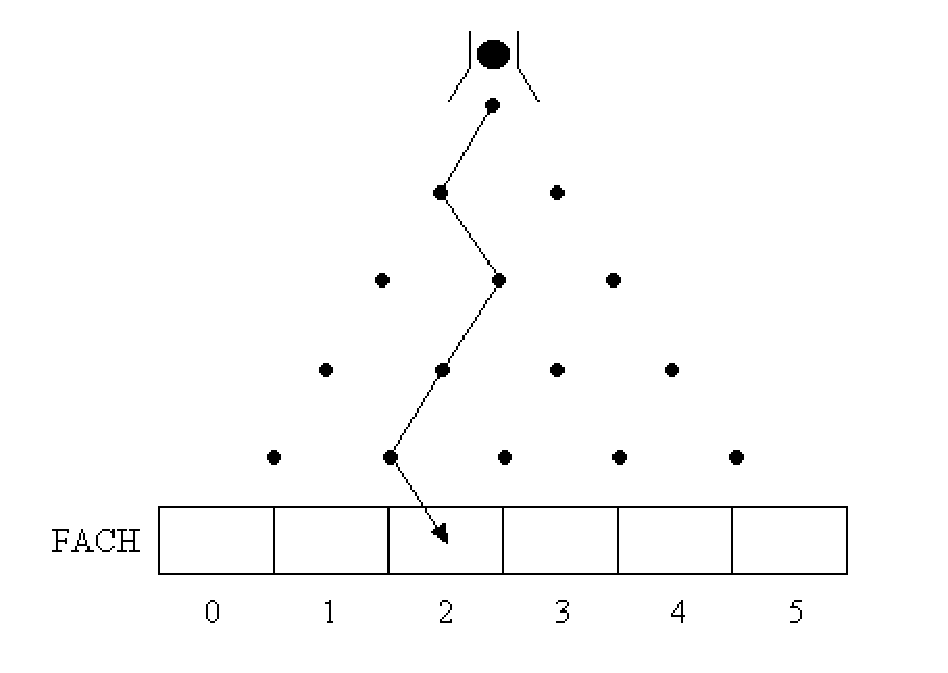
\includegraphics[width=200pt]{brett.eps}

\vspace{5mm}

Wir interessieren uns daf"ur, wieviele Kugeln in den einzelnen F"acher landen.\\
\\
Erstellen Sie ein Programm, welches mittels Simulation f"ur n=100 Kugeln die Verteilung auf die F"acher bestimmt.\\
\\
Ausgabe des Programms (keine Graphik):

\verbatiminput{brett.txt}

Beachten Sie, dass die Fach-Nr. einer Kugel gleich der Anzahl Rechtsablenkungen ist.
\end{document}

